\section{Git}\label{git-explanation}
This chapter introduces the \ac{vcs} \emph{Git}, as it plays a fundamental role in this thesis.
In the following the most relevant parts of Git will be explained such as user roles, technologies and internal data representations.
I will also talk about the current cases of application and some interesting scenarios which might be interesting for this thesis.


\subsection{Introduction to Git}\label{git-introduction}
At its core, Git is a tool, which is used to manage different versions of files in a specific directory. This
Each version of the project is saved as a so called \emph{commit}, which represents a specific state of all files and directories in the project.
Users are able to meticulously specify the files or changes in files that should be added to a commit, they can for example only select a subset of changes which happened.
By doing so one can split a large set of changes of possibly completely unrelated changes into several commits, where each commit forms a set of logically related changes.
Git is then capable of showing the exact changes between different commits, which is called a \emph{diff} and jumping between different versions of the project, which is called a \emph{checkout}.

Git is the currently most popular tool to control a project's code with a still trending tendency~\cite{article:git-popularity}.
It enables to work with multiple developers on a single code base, as it provides several different techniques, namely the history \emph{tree}, the \emph{branch} and the \emph{merge}.
The versioning history of Git is internally represented as an directed, non-cyclic, connected graph of commits or a tree.
The commits act as \emph{nodes} and the connection to their parent commits as \emph{edges}.
Every time two edges leave a single node, a new branch is created.
Git provides the feature to name branches, whereas the main branch is per default named \emph{master}.

\begin{figure}[H]
    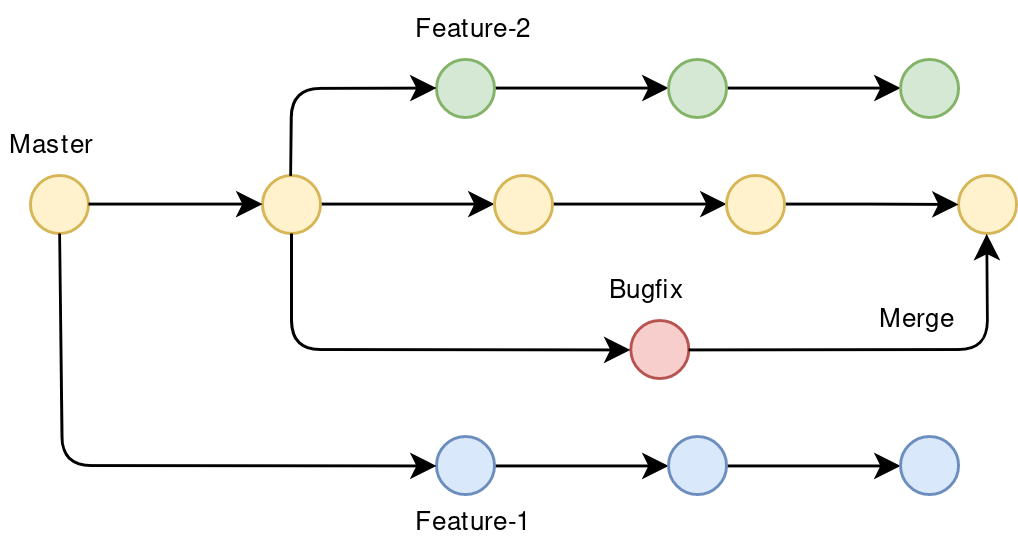
\includegraphics[scale=0.35]{./graphs/git-history-branch}
    \centering
    \caption{A Git commit history tree.}\label{fig:git-commit-tree}
\end{figure}

As shown in figure~\ref{fig:git-commit-tree} two developer can for example create their own branch on which they can work unimpeded.
If they finished a task and want to add their work to the master branch, they can now merge their changes.
Git then tries to automatically resolve any conflicts which might have emerged from editing the same lines in a file, if that is not possible, it marks the conflicts and allows the user to manually correct them.
After this resolution a new \emph{merge commit} is created. This merge commit represents the merge of the changes of two different branches.

With this methodology it is possible to work with many people or teams on the same project, without accidentally overwriting changes of another developer, whilst maintaining a clear history of all changes in the project.

Another important feature of Git is the possibility to set up a \emph{remote}.
A remote acts as a single source of truth a developer can \emph{push} their changes to or \emph{pull} changes from other developers.
It can for example be a distinct server, which is attached to some kind of network that is accessible by the developers.
This feature allows developers to distribute to a project, as long as they have access to this network.
Git also supports several protocols such as \ac{http} or \ac{ssh} to connect to the remote and to provide a simple user management layer.


\subsection{Git User Roles}
There exist two roles in Git, namely the \emph{committer} and the \emph{author}.
Every commit in Git contains the email addresses and the names of these two people.
The author of a commit is the person which actually contributed the changes in the files.
The committer is the person, which created the git commit.
This is important to keep track of the original author of the changes.

Lets look at the case of an author contributing code to a project in an email with an attached patch file.
If a maintainer of the project now applies the patch file and commits without setting the author, the information about the original author would be lost.
Collected data indicates that in about 89\% the author and the committer are the same person.


\subsection{Internal Representation}
Git underlying storage and management solution for files is commonly described as an mini filesystem~\cite[p.~9]{book:pro-git}, thereby I will refer to this as an \ac{fs} from now on.
Git provides a collection of high level abstraction tools to work with it's underlying \ac{fs}.
In the following I will explain the most important aspects of Git's \ac{fs} structure and management.

The representation of a single file in Git is a called \emph{blob} object~\cite[p.~56]{book:pro-git}.
A blob object is a file, which has been added to a Git \ac{fs}.
It is compressed and saved in the \inlinecode{.git/objects} directory under the respective \ac{sha1} hash of the uncompressed file.
As follows there exists a blob object for every version of every file of the project.

The \ac{sha1} hashing for unique file identifier might seem unsafe at first, but the probability of a \ac{sha1} collision is really low, roughly $10^{-45}$.
Lately Google managed to force a collision in an controlled environment in 2017, but it is really unlikely to encounter a collision under normal circumstances~\cite{techreport:sha-collision}.
This characteristic of \ac{sha1} hashing will become quite important in the design of the database later on.

As mentioned in the introduction~\ref{git-introduction} Git is used to store the state of a specific directory on any underlying \ac{os} \ac{fs}.
To represent a \ac{fs} or to simply bundle multiple Git blob objects together, Git uses the tree object.

A tree object is a file, which has a \ac{sha1} hash reference to all underlying blob and tree objects as well as their names and file permissions.
To represent a subdirectory a tree simply holds a reference to another tree object.
With these tools git manages to build it's own basic representation of a file system.

\begin{minted}[linenos]{text}
    100644 blob 11d1ee77f9a23ffcb4afa860dd4b59187a9104e9  .gitignore
    040000 tree ac0f5960d9c5f662f18697029eca67fcea09a58c  expose
    100644 blob 61b5b2808cc2c8ab21bb9caa7d469e08f875277a  install.sh
    040000 tree 8aaf336db307bdcab2f082bd710b31ddb5f9ebd4  thesis
\end{minted}
\begingroup
\captionof{listing}{A tree file example\label{lst:raw-commit}.}
\endgroup

As stated before the commit is utilized to provide an exact representation of a state of the repository's files and directories.
Just as blob object, the tree and commit files are also stored in the \inlinecode{.git/objects} directory under their respective hash.

\begin{minted}[linenos]{text}
    tree      cd7d001b696db430b898b75c633686067e6f0b76
    parent    c19b969705e5eae0ccca2cde1d8a98be1a1eab4d
    author    Arne Beer <arne@twobeer.de> 1513434723 +0100
    committer Arne Beer <arne@twobeer.de> 1513434723 +0100

    Chapter 2, acronyms
\end{minted}
\begingroup
\captionof{listing}{A commit file example\label{lst:raw-commit}.}
\endgroup

As you can see in listing~\ref{lst:raw-commit}, the commit is just another kind of file utilized by Git, which contains some metadata about a repository version:

\begin{itemize}
    \item The reference to a tree object, which represents the root directory of the commit's version of the project.
    \item A reference to one or multiple parent commits, to maintain a version history.
    \item The name and email address of the author.
    \item The name and email address of the committer.
    \item The \ac{utc} timestamps with \ac{utc} offset for the commit and author date.
    \item The commit message. A message with arbitrary text from the committer.
\end{itemize}

The commit is the most important object for this thesis.
It contains crucial information such as the date of the commit as well as the email, which is needed to identify a contributor across several commits.


\subsection{More features}

Git provides many more features, which are not necessarily important for data analysis, but which might be taken into account when aggregating the data.
In the following some functionalities will be shown, which can lead to problems or irregularities in the gathered data.

\begin{description}
    \item[rebase] \hfill \\
        It is possible to \emph{rebase} branches. For instance a rebase can rewrite the commit history and change the branch point of a branch to another commit.
        This is for example a very powerful but also dangerous tool, as it implicitly changes the timestamps of the commits of the rebased branch.

    \item[force push] \hfill \\
        Git allows to push to a remote with the \inlinecode{--force} flag, which is called a \emph{force push}.
        This enables the users to rewrite every commit in the whole history tree. If another user has a git repository version

\end{description}




